% !TeX root = RJwrapper.tex
\title{\pkg{markovMSM}: An R Package for Checking the Markov Condition in Multi-State Survival Data}
\author{by Gustavo Soutinho and Lu\'{i}s Meira-Machado}

\maketitle

\abstract{
Multi-state models can be used to describe processes in which an individual moves through a finite number of states in continuous time. These models allow a detailed view of the evolution or recovery of the process and can be used to study the effect of a vector of explanatory variables on the transition intensities or to obtain prediction probabilities of future events after a given event history. In both cases, before using these models, we have to evaluate whether the Markov assumption is tenable. This paper introduces the \CRANpkg{markovMSM} package, a software application for R, which considers tests of the Markov assumption that are applicable to general multi-state models. Three approaches using existing methodology are considered: a simple method based on including covariates depending on the history; methods based on measuring the discrepancy of the non-Markov estimators of the transition probabilities to the Markovian Aalen-Johansen estimators; and, finally, methods that were developed by considering summaries from families of log-rank statistics where individuals are grouped by the state occupied by the process at a particular time point. The main functionalities of the \CRANpkg{markovMSM} package are illustrated using real data examples.
}

\section{1. Introduction} \label{sec:intro}
%\section[Introduction]{1. Introduction} \label{sec:intro}

Multi-state models are commonly used to analyze complex longitudinal survival data involving multiple events of interest (\citealp{Andersen1993}; \citealp{Hougaard2000}; \citealp{Putter2007}; \citealp{MM2009}; \citealp{LFMM2019}). These models can be considered as a generalization of the survival process where survival is the ultimate outcome of interest, but where information is available about intermediate events that individuals may experience during the study period. For instance, in some biomedical applications, besides the 'healthy' initial state and the absorbing `dead' state, one may observe intermediate (transient) states based on health conditions (e.g., heart or lung disease), disease stages (e.g., stages of cancer, HIV infection or Alzheimer's), clinical symptoms (e.g., bleeding episodes), biological markers (e.g., CD4 T-lymphocyte cell counts; serum immunoglobulin levels) or they can represent a non-fatal complication in the course of the illness (e.g., cancer recurrence, transplantation, etc.). The number of states and transitions among them defines the complexity of the model, which is illustrated by a directed graph with rectangular boxes representing possible states and arrows representing the allowed transitions. Among the multi-state models, the simplest is the mortality model for survival data (with only two states). The competing risks model (\citealp{Andersen2002}; \citealp{Putter2007}) can be seen as an extension of the simple mortality model for survival data in which each individual may `die' due to any of several causes. The most common is the illness-death model, also known as the disability model, which comprises three states. In the irreversible version of this model (Figure 1), individuals start in the `alive and disease-free' state and subsequently move either to the `diseased' state or to the `dead' state. Individuals in the `diseased' state will eventually move to the `dead' state, without any possibility of recovery. Data that arises from the model depicted in Figure 1 has been termed as semi-competing risk data and can be seen as an emerging challenge for time-to-event data where two events of interest are studied: non-terminal (e.g., disease diagnosis) and terminal (e.g., death) events. The non-terminal event is observed only if it precedes the terminal event, which may occur before or after the non-terminal event. In this context, the terminal event is a competing risk for the intermediate state but not the contrary (\citealp{Xu2010}; \citealp{Li2017}; \citealp{Nevo2020}).

%{\color{blue} Figure 1 can also be viewed as a semi-competing risks model. In these models there are a nonterminating event (`disead') and a terminating event (`dead'). The non-terminal event is observed only if it precedes the terminal event, which may occur before or after the non-terminal event. In this context, the terminal event is a competing risk for the intermediate state but not the contrary (\citealp{Li2017}, \citealp{Nevo2020}).}

Multi-state models can be used to assess the effects of covariates on the transition intensities, but they can also be used to obtain conditional prediction probabilities of future events. From the transition intensities, it is possible to evaluate the probability of one event ahead, but the transition probabilities are the relevant predictive quantities since they consider several transitions ahead. The occupation probabilities, often used in practice, are particular examples of transition probabilities in which the time origin is taken as the current time. When the underlying stochastic process is Markov, an elegant theory can be used to link the transition intensities to the transition probabilities, leading to the Aalen-Johansen estimator \citep{AJ1978}. This assumption claims that given the present state, the future evolution of the process is independent of the states previously visited and the transition times among them; in other words, the history of the process is summarized by the current state. The Aalen-Johansen estimator is adapted to censoring, and benefits from the assumption of Markovianity to get consistent estimates. However, when the multi-state model is non-Markov, this is no longer the case. In fact, there are many applications for which the Markov assumption may not be met; for example, the arrival time at the current state of the process often influences the transition intensities, leading to non-Markov structures (\citealp{Andersen2000}, \citealp{Andersen2002}). Although the Aalen–Johansen estimator may be used to consistently estimate occupation probabilities for non-Markov multi-state models \citep{Datta2001}, in general it provides biased estimators if the Markov assumption does not hold. To tackle this issue, \cite{MM2006} introduced, for the first time, estimators that do not rely on the Markov assumption. These authors showed the practical superiority of their estimators relative to the Aalen-Johansen estimator in situations in which the Markov condition is strongly violated. However, this approach has the drawback of requiring that the support of the censoring distribution contains the support of the lifetime distribution, otherwise they only report valid estimators for truncated transition probabilities. Recently, alternative estimators that are consistent regardless of the Markov condition and the referred assumption on the censoring support were proposed by \cite{AlvarezMM2015}. The idea behind the proposed estimators is to use a procedure based on differences between Kaplan-Meier estimators derived from a subset of the data, consisting of all subjects observed to be in a given state at a given time. The same idea of subsampling, combined with the Aalen-Johansen estimator, was later used by \citet{PutterSpitoni2018} to introduce new estimators which were termed landmark Aalen-Johansen.

In the multi-state setting, it is of practical interest to determine whether the Markov property holds within a particular data set. This information can be used to assess the validity of the transition probability estimates as well as the best option for performing inference on the transition intensities when one aims to relate the individual characteristics to the intensity rates through a multi-state regression model. This assumption is usually checked by including covariates depending on the history (\citealp{Kay1986}; \citealp{Andersen2000}; \citealp{Andersen2002}). For the progressive illness-death model, for example, the Markov assumption is particularly relevant for modeling the death transition after disease and, consequently, assessing whether this transition rate is affected by the time in the previous state. Alternative methods, based on a local Kendall's tau measuring the future-past association along time, were proposed by \citet{Girondo2012} and \citet{Girondo2016}. The method proposed by these authors can be used for three-state progressive and illness-death models, but the extension of this test to general multi-state models is not straightforward, and thus flexible methods that may be used in general models are required. A very recent work by \citet{Titman2020} considers new approaches for checking this assumption. In one of these approaches, local and general tests have been developed by considering summaries from families of log-rank statistics where individuals are grouped by the state occupied at varying initial time $s$. \citet{Chiou2018} also considered an equivalent problem to testing Markovianity (in the progressive illness-model) but involving tests for dependent truncation. Making use of the landmark approach, \citet{soutinho_machado2020} introduces new methods for checking the Markov assumption through a local and global test given by measuring the discrepancy between the Aalen-Johansen estimator and the landmark estimators (\citealp{AlvarezMM2015}, \citealp{PutterSpitoni2018}) that are free of the Markov condition.

There are some software packages available for multi-state survival analysis. A comprehensive list of the available packages in the Comprehensive R Archive Network (CRAN) can be seen in the CRAN task view 'Survival Analysis' \citep{Allignol2018}. In particular, in the context of multi-state models, \CRANpkg{mstate} package provides functions for estimating hazards and probabilities, possibly depending on covariates. This package also permits checking the Markov assumption from families of log-rank statistics where individuals are grouped by the state occupied at different times \citep{Titman2020}. The \CRANpkg{msm} package can be used to fit a Markov model with any number of states and any pattern of transitions to panel data. It includes several extensions, such as hidden Markov models and models whose transition intensities vary with individual-specific or time-varying covariates \citep{Jackson2011}. \CRANpkg{survidm} package provides estimates of predictive probabilities, such as the transition probabilities, occupation probabilities, cumulative incidence functions, and waiting (sojourn) time distributions. It also allows one to perform multi-state regression for transition intensities as well as to implement global tests for the Markov assumption in illness-death models \citep{soutinho2021}. Other examples are the \CRANpkg{SemiMarkov} package that can be used to fit semi-Markov multistate models to longitudinal data proposed by \cite{Krol2015} and the \CRANpkg{frailtyEM} which contains functions for fitting shared frailty models with a semi-parametric baseline hazard with the Expectation-Maximization algorithm \citep{Balan2019}. Multi-state regression can be performed using several of the aforementioned packages by decoupling the whole process into various survival models, by fitting separate intensities to all permitted transitions using, for example, semi-parametric Cox proportional hazard regression models, while making appropriate adjustments to the risk set. To this end, the \CRANpkg{JM} and \CRANpkg{joineR} packages, proposed by \cite{JM} and \cite{joineR}, can be useful to estimate the parameters for the joint modeling of longitudinal and time-to-event data. In this context, we can also refer to the \CRANpkg{joineRML} which extends the inference of the joint model to the case of multiple continuous longitudinal measures \citep{joineRML}.

The organization of this paper is as follows: In Section 2, we present a brief introduction of the notation and the mathematical background of existing methods for testing the Markov assumption. In Section 3, we introduce the \CRANpkg{markovMSM} package, a software application for R that performs these local and global tests in the multi-state models described in \cite{soutinho_machado2020} using three real data examples. Finally, the main conclusions are reported in Section 4.

\begin{figure} [t] %[!ht]
\centering
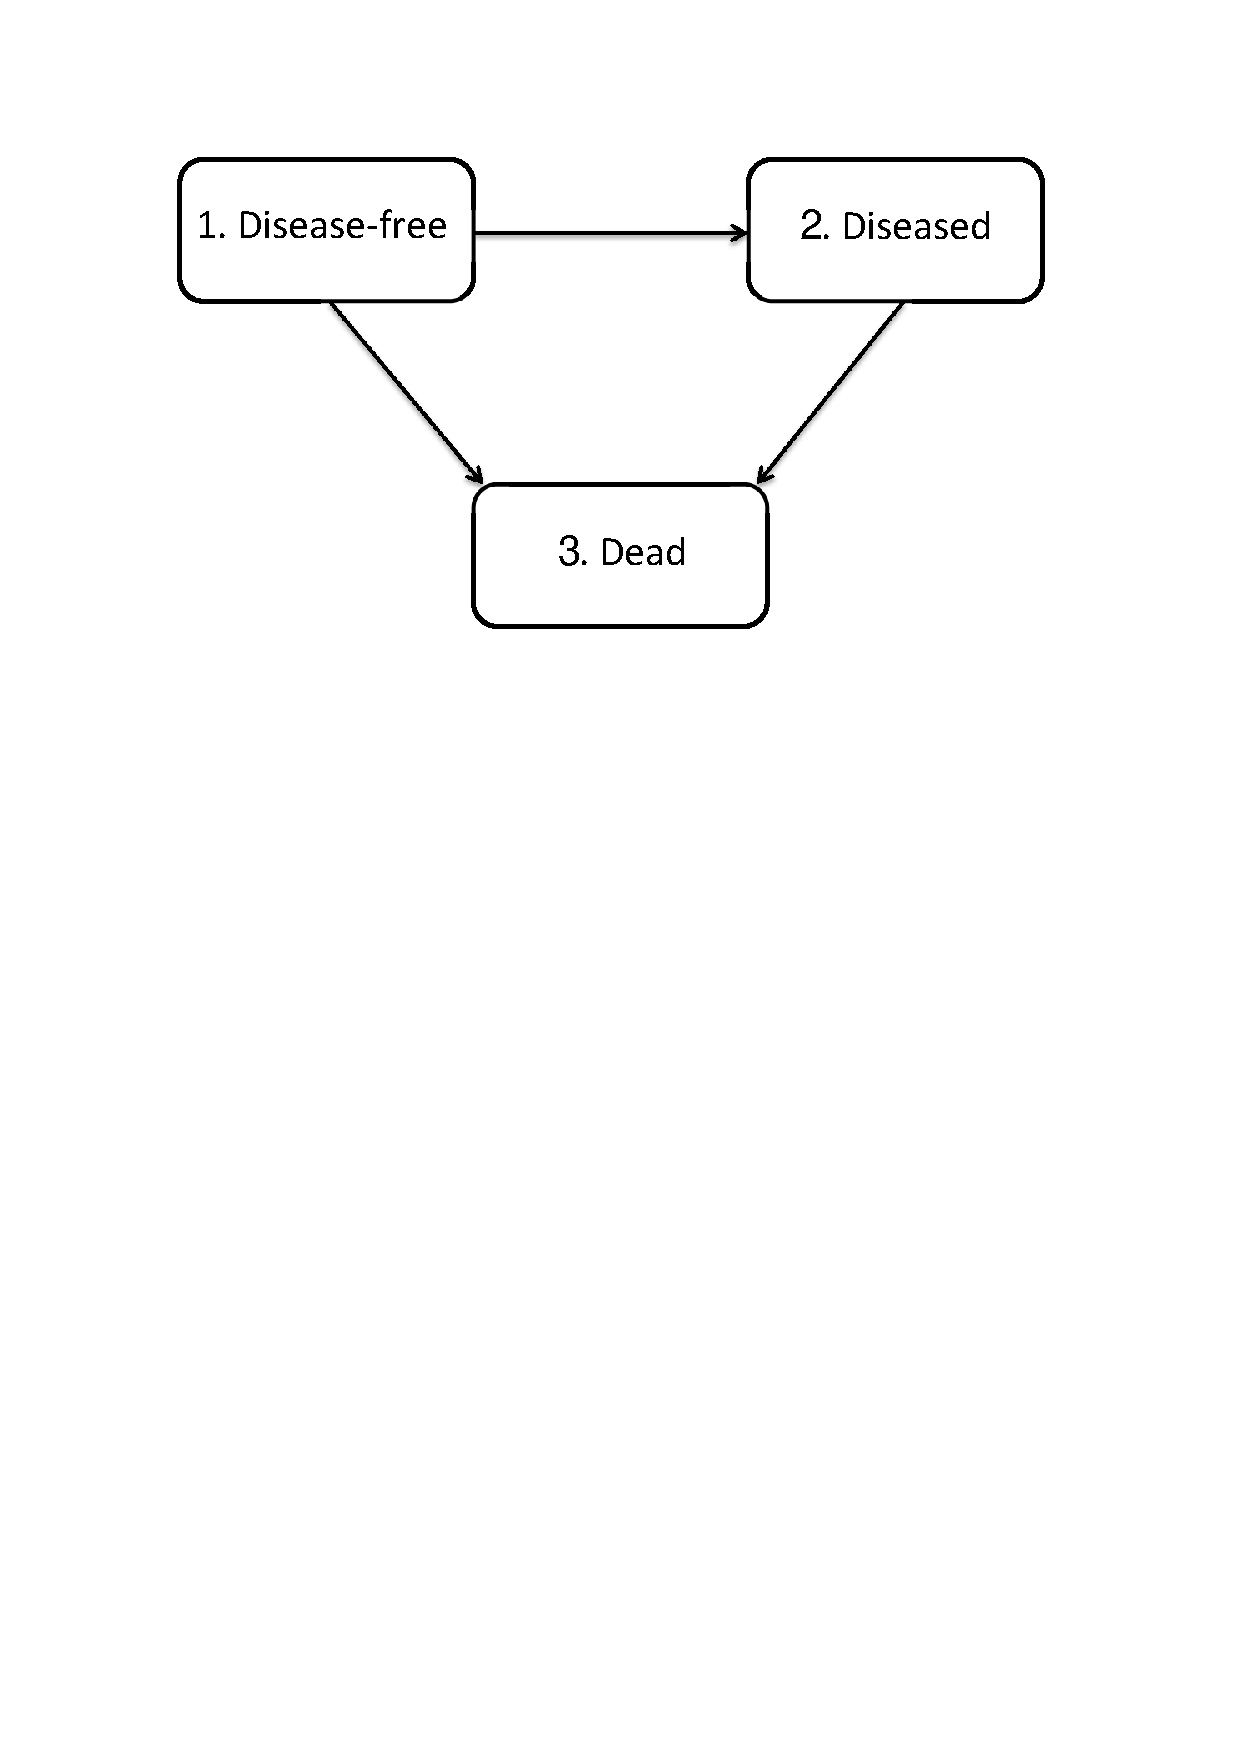
\includegraphics[width=6cm]{illness-death.pdf}
\caption{\label{IDM} The progressive illness-death model with three states and three irreversible transitions. `Disease-free` correspond to the initial state, `Diseased` the intermediate state and the absorbing state `dead`.}
\end{figure}


\section{2. Background and notation} \label{sec:methodology}

This section contains a brief description of the mathematical background underlying the \CRANpkg{markovMSM} package. Further details on the proposed methods can be found in \cite{soutinho_machado2020}.

\subsection{Multi-state models and transition probabilities} \label{multi}
A multi-state model $(X(t),t\in [0,\infty))$ is a model for a time continuous stochastic process. These models provide a relevant modeling framework for dealing with complex longitudinal survival data, since they allow the representation of the movement of the individuals among a set of finite states space $\mathcal{S}={1,\ldots ,K}$. They can be fully characterized through the transition probabilities, for two states $h$, $j$ and two time points $s < t$, that are given by the conditional probability $p_{hj}(s,t)=P(X(t)=j|X(s)=h, \mathcal{H}_{s-})$, where $\mathcal{H}_{s-}$ denotes the history of the process up to time $s$. This history can represent information about the process, such as the states previously visited, transition times, etc. Under the Markov assumption, $P(X(t)=j|X(s)=h, X(u)=y)=P(X(t)=j|X(s)=h)$, for any $0\leq u<s$ and $y \in \mathcal{S}$, and thus, the future of the process after time $s$ depends only on the state occupied at time $s$, not on the arrival time to that state or on the states previously visited.  

Without loss of generality and for the purpose of simplicity, let us consider the progressive illness-death model, with state space $\{1,2,3\}$, given by the initial State (e.g., `alive and disease-free'; State 1), the intermediate state (e.g., `diseased'; State 2), and the absorbing state (e.g., `dead'; State 3). For this type of model, there are five different transition probabilities to be considered that can be obtained as follows \citep{LFMM2019}:
\begin{center}
$p_{11}(s,t) = \exp\left(-\int_s^t \left(\lambda_{12}(u)+\lambda_{13}(u)\right)du\right)$
\end{center}
\begin{center}
$p_{22}(s,t\mid t_{12})= \exp\left(-\int_s^t \lambda_{23}(u,
t_{12})du\right)$
\end{center}
\begin{center}
$p_{12}(s,t) =\int_s^t p_{11}(s,u-)\lambda_{12}(u)p_{22}(u,t\mid
u)du$.
\end{center}
\noindent Here, $p_{22}(s, t\mid t_{12})$ denotes the transition probability $p_{22}$ conditional on a particular entry time $t_{12}$, and $\lambda_{hj}(.)$ correspond to the transition intensities that are the instantaneous hazards for movement from one state ($h$) to another ($j$). If the process is Markov, $h_{23}(t, t_{12})=h_{23}(t)$ and $p_{22}(s, t\mid t_{12})=p_{22}(s, t)$. The two other transition probabilities, $p_{13}(s,t)$ and $p_{23}(s,t)$, can be estimated from the two obvious relations that exist in the progressive illness-death model: $p_{11}(s,t)+p_{12}(s,t)+p_{13}(s,t)=1$ and $p_{22}(s,t)+p_{23}(s,t)=1$. Expressions for general models are not possible. Since the prognosis for an individual in the intermediate state may be influenced by the subject's specific arrival time, the illness-death model is not necessarily Markovian.

The estimation of the transition probabilities is a major goal in multi-state models since they allow for long-term predictions. A common nonparametric method to estimate these quantities is the Aalen-Johansen (\code{AJ}) estimator, \citep{AJ1978} which can be obtained as the product–integral of the Nelson-Aalen estimators for the cumulative transition intensities \citep{Andersen1993}. Explicit formulae of the Aalen-Johansen estimator for the illness-death model can be found in \cite{Borgan2005}. When the multi-state process is Markovian, the \code{AJ} estimator provides consistent estimates of the transition probabilities, but this is no longer the case if the process is non-Markov. To avoid this problem, \cite{AlvarezMM2015} use the idea of subsampling, also referred to as landmarking \citep{VanHouwelingen2007}, which is based on (differences between) Kaplan-Meier estimators derived from a subset of the data consisting of all subjects observed to be in the given state at the given time. For the specific case of the illness-death model, given the time point $s$, to estimate $p_{1j}(s,t)$ for $j=1,2,3$ the landmark analysis is restricted to the individuals observed in State 1 at time $s$; whereas, to estimate $p_{2j}(s,t)$, $j=2,3$, the landmark analysis proceeds from the sample restricted to the individuals observed in State 2 at time $s$. Further details on the formulae and proofs can be seen in \cite{AlvarezMM2015}.
The subsampling approach was later used by \citet{PutterSpitoni2018} to derive a landmark Aalen-Johansen estimator (\code{LMAJ}) of the transition probabilities. The idea behind the proposed estimator is to use the Aalen-Johansen estimator of the state occupation probabilities derived from those subsets (consisting of subjects occupying a given state at a particular time) for which consistency has already been proved in multi-state models that are not necessarily Markov \citep{Datta2001}. It is worth mentioning that, in the illness-death model, the landmark Aalen-Johansen estimators (\code{LMAJ}) and the landmark estimators (\code{LM}) of the transition probabilities have shown similar performances. However, the former methods (\code{LMAJ}) can be used in general multi-state models, which can be considered an advantage.

From now on, we will use the abbreviation \code{AJ} for the Aalen-Johansen estimator, \code{LM} for the LandMark estimator proposed by \cite{AlvarezMM2015}, and \code{LMAJ} for the LandMark Aalen-Johansen estimator \citep{PutterSpitoni2018}.

\subsection{Tests for the Markov assumption} \label{sec2.3}

\textit{\textbf{Modeling particular transition intensities}}\\\\
%\subsubsection{Modeling particular transition intensities}
Traditionally, the Markov condition is verified by modeling particular transition intensities on aspects of the history of the process using a proportional hazard model (\citealp{Kay1986}; \citealp{Andersen2000, Andersen2002}). In the progressive illness-death model, the Markov condition is particularly relevant for the transition from the intermediate state `disease' (State 2) to `death' (State 3). Under this model, we can examine whether the time spent in the initial state (State 1) is important in the transition from the disease state to death or not. For doing that, let $\lambda_{23}(t)$ denote the hazard function of $T$ for those individuals going from State 2 to State 3. Fitting a Cox model $\lambda_{23}(t\mid Z)=\lambda_{23,0}(t)\exp(\beta Z)$, where $\lambda_{23,0}$ is the baseline hazard, $Z$ the `time spent in the healthy (initial) state' and $\beta$ a regression parameter, we now need to test the null hypothesis, if the transition rate from the disease state into death is unaffected by the time spent in the healthy state, $H_0:\beta=0$, against the general alternative, $H_1:\beta\neq 0$. This `global' test, based on the semiparametric Cox proportional hazards model, assumes proportional hazards and a linear effect on the hazard for the covariate. When either of these two assumptions is not fulfilled, the test may not be able to detect the lack of Markovianity. 

Since the landmark methods (\code{LM}) for estimating the transition probabilities proposed by \cite{AlvarezMM2015}, and (\code{LMAJ}) by \cite{PutterSpitoni2018} are free of the Markov assumption, they can be used as a basis for the construction of tests for Markovianity. These ideas were used by \cite{soutinho_machado2020} to introduce local and global tests for Markovianity based on the discrepancy of the landmark estimators to Markovian Aalen-Johansen estimators (\code{AJ}). Subsampling, also known as landmarking, has been also used by \cite{Titman2020} to introduce a general test based on summaries from families of log-rank statistics where individuals are grouped by the state they occupied at a given (landmark) time.\\

\textit{\textbf{AUC Local Test}}\\\\
%\subsubsection{AUC Local Test}
\cite{soutinho_machado2020} introduce a local test based on the area under curve, AUC, given by the estimated transition probabilities, for a fixed time $s>0$, that can be used for a general multi-state model for checking the Markovianity of the process. They propose the following test statistic that is based on the difference between the area under the estimated transition probability curve for the non-Markov \code{LMAJ} estimator and the \code{AJ} estimator, $U=\int_{s}^{\tau}
\left(\widehat p_{hj}^{\texttt{ LMAJ}}(s,u) - \widehat p_{hj}^{\texttt{ AJ}}(s,u)\right)du$, where $\tau$ is the upper bound of the support of $T$. When the process is Markovian, it is expected that the test statistic will be close to zero. The Markov assumption becomes less likely as the test statistic gets further away from zero in either direction. Because of censoring, both estimators (\code{LMAJ} and \code{AJ}) may reveal high variability in the right tail, which may inflate the test statistic. In addition to this issue, since landmarking is based on reduced data, the maximum point for which the \code{LMAJ} transition probability estimate is strictly defined may be lower than the maximum point for \code{AJ}. To address these issues, we propose that when computing $U$, the minimum between the upper bound for which \code{LMAJ} is defined and the 90\textit{th} percentile of the total time for the upper limit in the integral that defines the test statistic be used.

In the progressive illness-death model, besides the transition probability $\widehat p_{23}(s,t)$, $\widehat p_{12}(s,t)$ can also be used to test the Markov assumption. For general multi-state models, one can use transitions depending on history. In fact, if the goal is to decide which estimator is the most appropriate to use to estimate a specific transition probability $p_{hj}(s,t)$, then the test statistic should be the one based on that same transition probability.

To approximate the distributions of the test statistic, bootstrap methods with a large number of resamples, $M$, are used. We generate $M$ bootstrap samples, and for each sample, we calculate the test statistic $U^{\star}$ which corresponds to the difference between the areas of the \texttt{AJ} and the \texttt{LMAJ} estimators. Finally, the variance $\sigma^{\star}_{(U^{\star})}$ is obtained from the $M$ values of $U^{\star}$. Then, according to large sample asymptotic distribution theory, when $M$, the number of replicates, goes to infinity, we have the following statistic distributed approximately as a standard normal distribution with a mean of 0 and variance of 1:
$V=(U-0)/\sigma^{\star}_{(U^{\star})}\sim N(0,1)$. The null hypothesis will be rejected if $V>v_{(1-\alpha/2)}$ or $V<v_{(\alpha/2)}$, where $v_{(\alpha/2)}$ and $v_{(1-\alpha/2)}$ denote the $\alpha/2$ and $1-\alpha/2$ percentiles, respectively, of a normal distribution with a mean of 0 and variance of 1.\\

\textit{\textbf{AUC Global Test}}\\\\
%\subsubsection{AUC Global Test}
\cite{soutinho_machado2020} also introduce a global test, which can be achieved by combining the results obtained from local tests over different times. The testing procedure used here involves the following steps:

\begin{enumerate}

\item Using the original sample of the illness-death model, obtain the percentiles 5, 10, 20, 30, and 40 of the times spent by all individuals in State 1, the so-called waiting (soujorn) time. For general multi-state models, we recommend the use of the same percentiles of the subject's specific arrival time at the corresponding state.

\item For each of the values $s$ obtained in Step 1, obtain the probability values for the local method as explained before.

\item Obtain the mean of the probability values for each closest pair; i.e., the mean of the probability values of the following pairs of percentiles: $(5,10)$, $(10,20)$, $(20,30)$ and $(30,40)$.

\item Finally, the \textit{p}-value for the global test is equal to the minimum between the four probability values obtained in Step 3. In the case of this probability value being below a particular significance value, for example $0.05$, we reject the null hypothesis of the process being Markovian.
\end{enumerate}

Step 1 considers a global test based on local tests computed at low percentiles of subject-specific arrival times at the corresponding state. This is based on our experience that the failure of Markovianity often occurs at small transition times. Besides the hypothesis tests proposed above, we also suggest graphical local tests that can be used to check the Markov assumption in the illness-death model as well as for more complex multi-state models, possibly with reversible transitions between states. These graphical tests can be used to validate the default values proposed in Step 1 or to propose alternative values for which a discrepancy between the two methods (\code{LMAJ} and \code{AJ}) is more evident. 

The procedure described in Step 3 can be used to ensure that there is a discrepancy between the two estimated curves over a large range of time values.\\

\textit{\textbf{Log-rank test}}\\\\
%\subsubsection{Log-rank test}
%{\color{red} incluir algo sobre o teste de log-rank local e global. Buscar nas publicacoes de Putter e Titman}
The construction of the landmark Aalen-Johansen estimators (\code{LMAJ}) also motivated the development of new tests of the Markov assumption \citep{Titman2020}. Assume initially that interest lies in assessing the validity of transition probability estimates from a specific
start point time $s$ and a given state $h$, i.e. $p_{hj}(s,t)$. Under the landmark approach, the estimators of the transition probabilities should be derived from the subset of the data consisting of all subjects observed to be in the state $h$ at time $s$, $S=\{i:X_i(s)=j, Y_i(s)=1\}$ where $Y_i(s)$ is the at risk indicator of the process (\citealp{AlvarezMM2015}; \citealp{PutterSpitoni2018}). On the other hand, the Aalen-Johansen estimator would use also the set of subjects in $S^c=\{i:X_i(s)\neq j, Y_i(s)=1\}$. Besides, under a Markov process, the transition intensities of the process for $t>s$ will be the same in the two groups. This motivated \cite{Titman2020} to propose a local test for the Markov assumption that lies in testing $H_0: \lambda(t|X(s)=h)= \lambda(t|X(s)\neq h)$ for $t\geq s$ versus a general alternative. The proposed test is constructed using several log-rank statistics grouped by membership in $S$. \cite{Titman2020} also propose a global test via a grid of times in which, for each $s$ time, local tests are computed. In this paper, the grid of values is given by the percentile times.

%The construction of the landmark Aalen-Johansen estimators (LMAJ) also motivated the development of new tests of the Markov assumption (Titman and Putter 2020). Suppose initially that interest lies in assessing the validity of transition probability estimates from a specific start point time $s$ and state $j$. Under the landmark approach, the estimators of the transition probabilities should be derived from the subset of the data consisting of all subjects observed to be in the state $j$ at time $s$, $S={i:X_i(s)=j}$. Ver atigo Titman e Putter

%The idea of subsampling, also known as landmarking, combined with the Aalen–Johansen estimate of the state occupation probabilities derived from that subset, was also used by Putter and Spitoni (2018) to introduce the termed landmark Aalen-Johansen estimators. The estimators

%estimators derived from a subset of the data consisting of all subjects observed to be in the given state at the given time.

%A log-rank statistic for each transition from State $l$ to State $m$ is then of the form

%GLOBAL TEST  Titman and Putter (2020) 
The same authors pointed out that the use of the individual supremum or integrated statistics may be combined to provide an overall test of the dependence of the transition intensities on occupation in state $j$ at previous times. 

%extended the aforementioned log-rank local test to the general illness–death model, and they propose a global supremum-type statistic by considering the

%The individual supremum or integrated statistics may be combined to provide an overall test of dependence of the transition intensities on occupation in state j at previous times. Moreover

%This can be achieved by combining the individual log-rank test statistics over different transitions, as well as over qualitative states ℓ and time s. This

\section[Application of the markovMSM]{3. Application of the \pkg{markovMSM}} \label{sec: package}

This section offers the guidelines for the use of the \CRANpkg{markovMSM} package with the R statistical program \citep{R}. To this end, a description of the functions of the package is illustrated using three real data sets. The first one involves data from a clinical trial on colon cancer modeled using the progressive illness-death model \citep{Moertel1995}. Extensions to progressive processes beyond the three-state illness-death model are demonstrated using data from the European Group for Blood and Marrow Transplantation (EBMT) \citep{Putter2007}. Finally, we use data from a study with liver cirrhosis patients subjected to prednisone treatment \citep{Andersen1993}. The package comprises seven main functions, which are briefly summarized in Table~\ref{Tab1}.  

\subsection{Data manipulation} \label{sec:conc}

In this section, we reanalyze data from a large clinical trial on Duke's stage III patients affected by colon cancer who underwent curative surgery for colorectal cancer \citep{Moertel1990}. Of the 929 patients, 468 developed a recurrence, and among these, 414 died; 38 died without a recurrence. The remaining 423 patients were alive and disease-free up to the end of the follow-up. Besides the two event times (time to recurrence and time to death) and the corresponding indicator statuses, a vector of covariates including age, sex, number of lymph nodes, and extent of local spread is also available. Below is an excerpt of the data set with one row per individual. Individuals were chosen in order to represent all possible combinations of movements among the three states.

%\begin{CodeChunk}
%\begin{CodeInput}
\begin{example}
> library(markovMSM)
> data("colonMSM")
> db_wide <- colonMSM
> head(db_wide[c(1:2,16,21),1:11])

   time1 event1 Stime event      rx sex age obstruct perfor adhere nodes
1    968      1  1521     1 Lev+5FU   1  43        0      0      0     5
2   3087      0  3087     0 Lev+5FU   1  63        0      0      0     1
16  1323      1  3214     0     Obs   1  68        0      0      0     1
21  2789      0  2789     1     Obs   1  64        1      0      0     1
\end{example}
%\end{CodeInput}
%\end{CodeChunk}

\begin{table}[t!] %t: para fica no topo da pagisna %estava h
\begin{small}
\begin{tabular}{p{3.5cm}p{9.6cm}}
%\toprule
\hline
Function & Description \\
%\midrule
\hline
\code{PHM.test} & Performs a global test for the Markov assumption based on the Cox PH model.\\
\code{AUC.test} & Performs global and local tests for the Markov assumption using the Area Under Curves (AUC) method.\\
\code{LR.test} & Log-rank based test for the validity of the Markov assumption.\\
\code{plot.markovMSM} &  Plot for an object of class \code{markovMSM}.\\
\code{eventsMSM} &  Counts the number of observed transitions in the multi-state model.\\
\code{prepMSM} &  Prepares the data set for multi-state modeling in a long format from a data set in wide format.\\
\code{transMatMSM} &  Define transition matrix for a multi-state model.\\
\code{print.markovMSM} &  Print for an object of class \code{markovMSM}.\\
\code{summary.markovMSM} &  Summary for an object of class \code{markovMSM}.\\
\hline
%\bottomrule
\end{tabular}
\caption {Summary of functions in the \CRANpkg{markovMSM} package.}
\label{Tab1}
\end{small}
\end{table}

%{\color{red} Alterei o paragrafo em baixo. verificar se esta bem!}
%{\color{green2} Professor Luís, penso que está bem, em particular o facto de referir surgery. Ia colocar agora o seguinte texto, em que procuro indicar os possíveis estados a que se pode chegar (ou mesmo que se mantem no mesmo estado) a partir do estado inicial, o que representa a ideia para modelos mais complexos:

%\code{time1} represents the disease-free survival time or the transition times from the initial state to the attainable states: the intermediate state (recurrence) or the ultimate state (death). \code{event1} corresponds to the status/censoring indicator for the variable \code{time1}. The variable \code{Stime} represents the total survival time and \code{event} for its corresponding indicator status. }


The four initial variables describe the movement of the patients among the three states of the illness-death model: \code{time1} denote the time measured in days from surgery to recurrence, whereas \code{Stime} is the total time or the time to death or censoring; \code{event1} and \code{event} denote the corresponding status/censoring indicator (1 for an event and 0 for censoring). Patient 1 had a recurrence after 968 days (i.e., observed a transition from the initial state to the intermediate state) and then died after 1521 days in the study. Patient 2 remained alive and without recurrence at the end of follow-up (\code{event1 = 0} and \code{event = 0}). The two event times are equal in these cases. The patient represented in the third line had a recurrence after 1323 days but remained alive at the end of the follow-up (i.e., in State 2). Finally, the patient represented in the last line died after 2789 days in the study without experiencing a recurrence. 

%the variable \code{Stime} represents the total survival time and \code{event} for its corresponding indicator status. The individual represented in the first line experienced a recurrence of the tumor and have died. In these cases \code{event1 = 1} indicates that the individual observed a transition from State 1, whereas \code{event = 1} indicates that he reached the absorbing state (State 3). Since \code{time1 < Stime} then the individual observed a transition from State 1 to State 2. Individuals that observe a direct transition from State 1 to the absorbing state have a disease-free survival time that is equal to the death time (\code{time1 = Stime} with \code{event1 = 1} and \code{event = 1}). Individual represented in line 2 remain alive and without recurrence at the end of follow-up (\code{event1 = 0} and \code{event = 0}). Observations with \code{event1 = 1} and \code{event = 0} (and therefore with \code{time1 < Stime}), corresponds to individuals with an observed recurrence that remain alive at the end of the follow-up (i.e. State 2).  

As the original data set is in the wide format, the next step to implementing the proposed methods will be to convert the data into a long format, which is given by one line for each transition for which a subject is at risk. This can be done using functions \code{transMatMSM} and \code{prepMSM}. \code{transMatMSM} function defines the transition matrices, revealing which transitions are possible, whereas \code{prepMSM} provides a new dataset in a long format for which each row will correspond to a transition for which a patient is at risk. For the progressive illness-death model, these two functions are used as follows:

%\begin{CodeChunk}
%\begin{CodeInput}
\begin{example}
> positions <- list(c(2, 3), c(3), c())
> state.names <- c("Alive", "Rec",  "Death")
> tmat <- transMatMSM(positions, state.names)
> tmat
       to
from    Alive Rec Death
  Alive    NA   1     2
  Rec      NA  NA     3
  Death    NA  NA    NA
  
> timesNames <- c(NA, "time1", "Stime")
> status <- c(NA, "event1", "event")
> trans <- tmat
> db_long <- prepMSM(data = db_wide, trans, timesNames, status)
> db_long[1:10,]


   id from to trans Tstart Tstop time status
1   1    1  2     1      0   968  968      1
2   1    1  3     2      0   968  968      0
3   1    2  3     3    968  1521  553      1
4   2    1  2     1      0  3087 3087      0
5   2    1  3     2      0  3087 3087      0
6   3    1  2     1      0   542  542      1
7   3    1  3     2      0   542  542      0
8   3    2  3     3    542   963  421      1
9   4    1  2     1      0   245  245      1
10  4    1  3     2      0   245  245      0
\end{example}
%\end{CodeInput}
%\end{CodeChunk}

Finally, in terms of manipulation of data, a useful function is \code{eventsMSM} since it allows one to summarise the number of transitions among states and their percentages:

%\begin{CodeChunk}
%\begin{CodeInput}
\begin{example}
> eventsMSM(db_long)

$Frequencies
       to
from    Alive Rec Death no event total entering
  Alive     0 468    38      423            929
  Rec       0   0   414       54            468
  Death     0   0     0      452            452

$Proportions
       to
from        Alive       Rec     Death  no event
  Alive 0.0000000 0.5037675 0.0409042 0.4553283
  Rec   0.0000000 0.0000000 0.8846154 0.1153846
  Death 0.0000000 0.0000000 0.0000000 1.0000000
\end{example}
%\end{CodeInput}
%\end{CodeChunk}

\subsection{Methods for testing the Markov condition
in the illness-death model} \label{sec:mkv tests1}
The illness-death model is a special multi-state model with several applications in the biomedical literature. Many time-to-event data sets with multiple end points can be reduced to this generic structure. Unlike the survival or competing risk models, this model is not necessarily Markovian since the prognosis for an individual in the intermediate state may be influenced by the subject's specific arrival time. Traditionally, the Markov assumption is checked by including covariates depending on the history. In the particular case of the colon cancer data set, we are interested in assessing if the transition rate from the recurrence state into death is unaffected by the time spent in the previous state. This global test for the Markov assumption can be done using the function \code{PHM.test}. A brief description of the arguments of this function is shown in Table~\ref{Tab-PHM.test}. Results for this global test of our data indicated that the effect of the time spent in State 1 is not significant (\textit{p}-value of 0.154), revealing no evidence against the Markov model for the colon data. The corresponding input codes are the following:

%{\color{red} proponho alterar o nome da funcao Cox.globaltest para PHM.test. Mais,  em vez de colocarmos transition=3 que para o utilizador nao significa nada sugiro que a funcao seja construida para ler transition="23" ou ainda melhor, from=2, to=3. O res deve dar logo o p-value podendo o utilizador obter outra informação se quiser...}

%\begin{CodeChunk}
%\begin{CodeInput}
\begin{example}
> res <- PHM.test(data = db_long, from = 2, to = 3)
[1] 0.1543195
> res
$p.value
[1] 0.1543195
$from
[1] 2
$to
[1] 3
\end{example}
%\end{CodeInput}
%\end{CodeChunk}

\begin{table}[h]%[t!]
\begin{small}
\begin{tabular}{p{3.5cm}p{9.6cm}}
\hline
%\toprule
Argument & Description \\
\hline
%\midrule
\code{data} & A data frame in the long format containing the subject \code{id}; \code{from} corresponding to the starting state; the receiving state, \code{to}; the transition number, \code{trans}; the starting time of the transition given by \code{Tstart}; the stopping time of the transition, \code{Tstop}, and \code{status} (for the  status variable, with 1 indicating an event (transition), 0 a censoring).\\
\code{from} & The starting state of the transition to check the Markov 
condition.\\
\code{to} & The last state of the considered transition to check the 
Markov condition.\\
\hline
\end{tabular}
\caption {Summary of the arguments of the function \code{PHM.test}.}
\label{Tab-PHM.test}
\end{small}
\end{table}


In the \CRANpkg{markovMSM} package the local test proposed in Section \ref{sec2.3} is performed using function \code{AUC.test}, through argument \code{type='local'}. A summary of the arguments of this function is presented in Table~\ref{Tab3}. 

\begin{table}[t!]%[h]
\begin{small}
\begin{tabular}{p{3.5cm}p{9.6cm}}
%\toprule
\hline
Argument & Description \\
\hline
%\midrule
\code{data} & A data frame in the long format containing the subject \code{id}; \code{from} corresponding to the starting state; the receiving state, \code{to}; the transition number, \code{trans}; the 
starting time of the transition given by \code{Tstart}; the stopping time of the transition, \code{Tstop}, and \code{status} for the  status variable, with 1 indicating an event (transition), 0 a censoring.\\
\code{from} & The starting state of the transition probabilities.\\
\code{to} & The last receiving state considered for the estimation of the transition probabilities. All the probabilities among the first and the last states are also computed.\\
\code{type} & Type of test for checking the Markov condition: \code{local} or \code{global}. By default \code{type='global'}.\\
\code{times} & For the local test, times represents the starting times of the transition probabilities. In case of a global test, the argument is given by times between the minimum time and the third quartile times used in the formula of this test. Default to \texttt{NULL}.\\
\code{quantiles} & Quantiles used in the formula of the global test for the AUC methods.\\
\code{tmat} & The transition matrix for multi-state model.\\
\code{replicas} & Number of bootstrap samples to standardization of the T-statistic given by the difference of the areas of \code{AJ} and \code{LMAJ} transition probabilities estimates.\\
\code{limit} & Percentile of the event time used as the upper bound for the computation of the AUC-based test.\\
\code{positions} & List of possible transitions; x[[i]] consists of a vector of state numbers reachable from state i.\\
\code{namesStates} & A character vector containing the names of either the competing risks or the states in the multi-state model specified by the competing risks or illness-death model. names should have the same 
length as the list x (for \code{transMat}), or either $K$ or $K+1$ (for \code{trans.comprisk}), or 3 (for \code{trans.illdeath}).\\
\code{timesNames} & Either 1) a matrix or data frame of dimension $n \times S$ ($n$ being the number of individuals and $S$ the number of states in the multi-state model), containing the times at which the states are visited or last follow-up time, or 2) a character vector of length $S$ containing the column names indicating these times. In the latter cases, some elements of time may be \code{NA}\\
\code{status} & Either 1) a matrix or data frame of dimension $n \times S$, containing, for each of the states, event indicators taking the value 1 if the state is visited or 0 if it is not (censored), or 2) a character vector of length S containing the column names indicating these status variables. In the latter cases, some elements of status may be \code{NA}\\
%\bottomrule
\hline
\end{tabular}
\caption {Summary of the arguments of function \texttt{AUC.test}.}
\label{Tab3}
\end{small}
\end{table}


The input commands to perform the AUC local test, for a fixed time $s=180$ and transitions 1$\rightarrow$2 and 1$\rightarrow$3 are the following:

%\begin{CodeChunk}
%\begin{CodeInput}
\begin{example}
> set.seed(1234)
> res2 <- AUC.test(data = db_long, times = 180, from = 1, to = 3, type = 'local', 
                   replicas = 100, tmat = tmat)
> res2$localTest
    s    1->1        1->2        1->3
1 180 0.2902191 0.002982042 0.002992007
\end{example}
%\end{CodeInput}
%\end{CodeChunk}


As a result, the function \code{AUC.test} returns the probability values for all attainable transitions from the initial state. To obtain the same local test for transition 2$\rightarrow$3, we only need to put 2 in the parameter \code{from} as follows:

%\begin{CodeChunk}
%\begin{CodeInput}
\begin{example}
> set.seed(1234)
> res3 <- AUC.test(data = db_long, times = 180, from = 2, to = 3, type = 'local', 
                   replicas = 100, tmat = tmat)
> res3$localTest
    s     2->2         2->3
1 180  0.02547708   0.04816232
\end{example}
%\end{CodeInput}
%\end{CodeChunk}


Results reveal a possible failure of the Markov assumption with low probability values for transitions 1$\rightarrow$2 and 2$\rightarrow$3 for $s=180$ (less than 5\%). These findings agree with the results depicted in Figure~\ref{fig4}, which reports the estimated transition probabilities. In fact, we can observe departures between the two Markov-free estimators (\code{LM} and \code{LMAJ}) and the Aalen-Johansen estimator (\code{AJ}) revealing a possible failure of the Markov assumption. The input commands to obtain the plots shown in Figure~\ref{fig4} are the following:

%\begin{CodeChunk}
%\begin{CodeInput}
\begin{example}
> plot(res2, to = 2, axis.scale = c(0,0.25), difP = FALSE) #Figure 2 (Left column)
> plot(res3, to = 3, axis.scale = c(0,1), difP = FALSE) # Figure 2 (Right column)
\end{example}
%\end{CodeInput}
%\end{CodeChunk}

 
\begin{figure} [t] %[!ht]
\centering
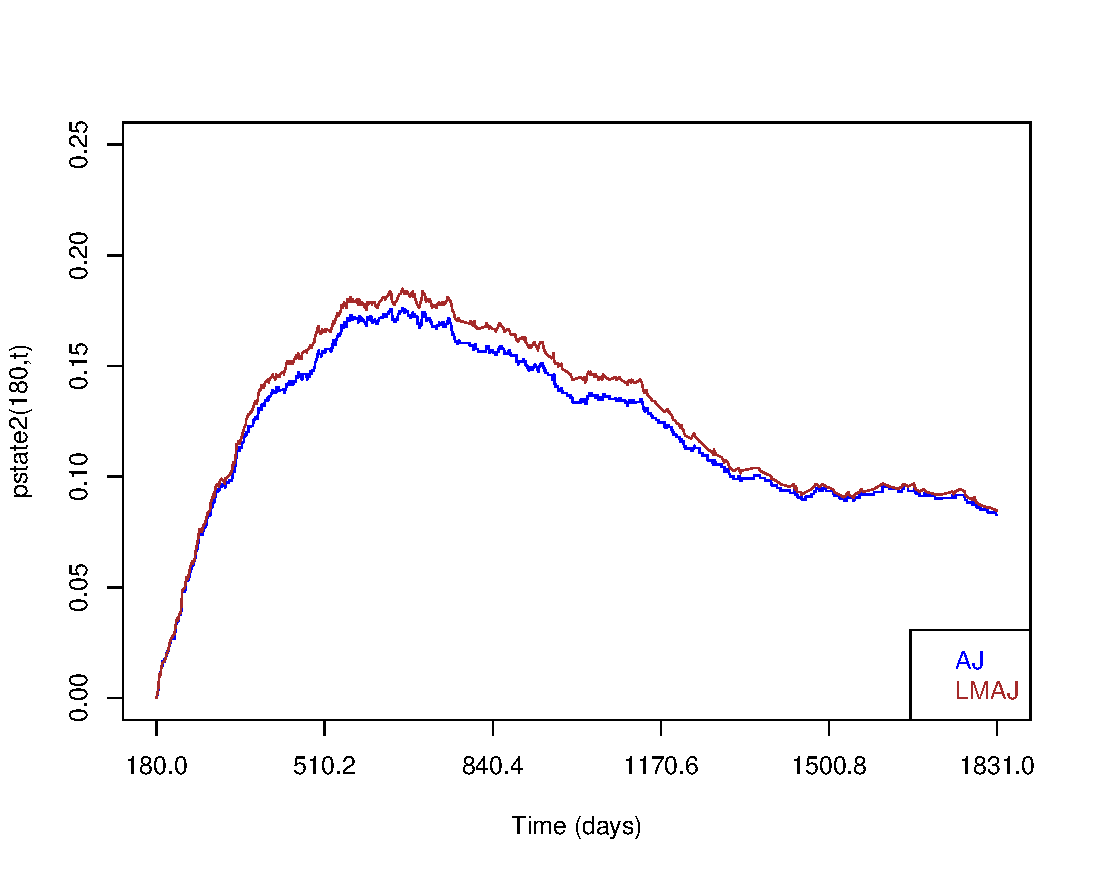
\includegraphics[width=6.5cm, height=6.5cm]{colon/p12_180_t_new2.pdf}
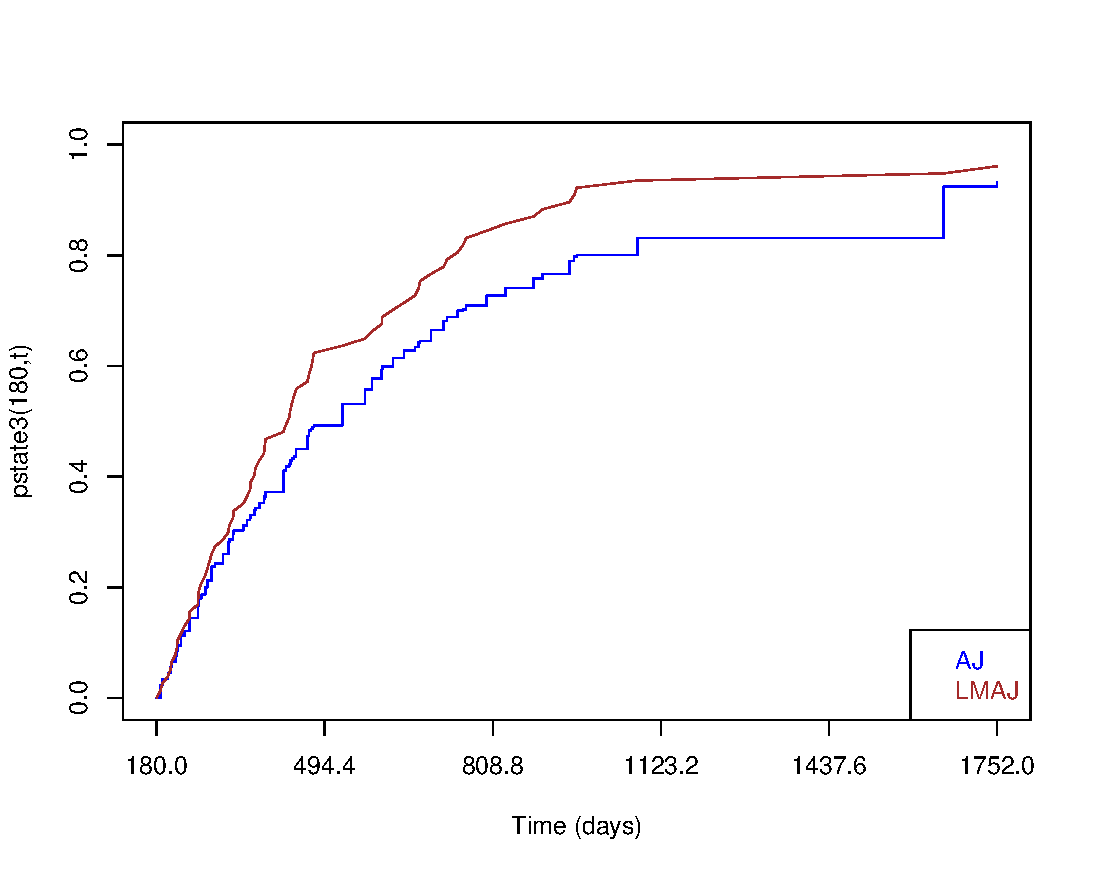
\includegraphics[width=6.5cm, height=6.5cm]{colon/p23_180_t_new2.pdf}\\

\caption{\label{fig4} Estimated transition probabilities for the Aalen-Johansen (\texttt{AJ}) and Markov-free estimators (landmark and landmark Aalen-Johansen) using data from a colon cancer for  $s = 180$. The displayed curves reveal a possible failure of the Markov assumption due to the departures between the \texttt{LM} and \texttt{AJ} estimates.}
\end{figure}

Putting the parameter \code{difP=TRUE}, we can also obtain the discrepancy between the Aalen-Johansen estimator (Markovian) and the landmark non-Markovian estimator (\code{LMAJ}), for $p_{12}(s,t)$ and $p_{23}(s,t)$, for $s=180$, measured through $D_{hj}=\widehat p_{hj}^{\texttt{AJ}}(s,t)-\widehat p_{hj}^{\texttt{ LMAJ}}(s,t)$, $h=1,2$, $j=h+1$. The 95\% pointwise confidence limits were obtained using a simple bootstrap (Figure~\ref{fig6}). The corresponding input commands in this case are the following:

%\begin{CodeChunk}
%\begin{CodeInput}
\begin{example}
> plot(res2, to = 2, axis.scale = c(-0.03,0.03), difP = TRUE) #Figure 3 (Left column)
> plot(res3, to = 3, axis.scale = c(-0.30,0.10), difP = TRUE) #Figure 3 (Right column)
\end{example}
%\end{CodeInput}
%\end{CodeChunk}


%PUT plot about here
\begin{figure} [t] %[h!]
\begin{center}
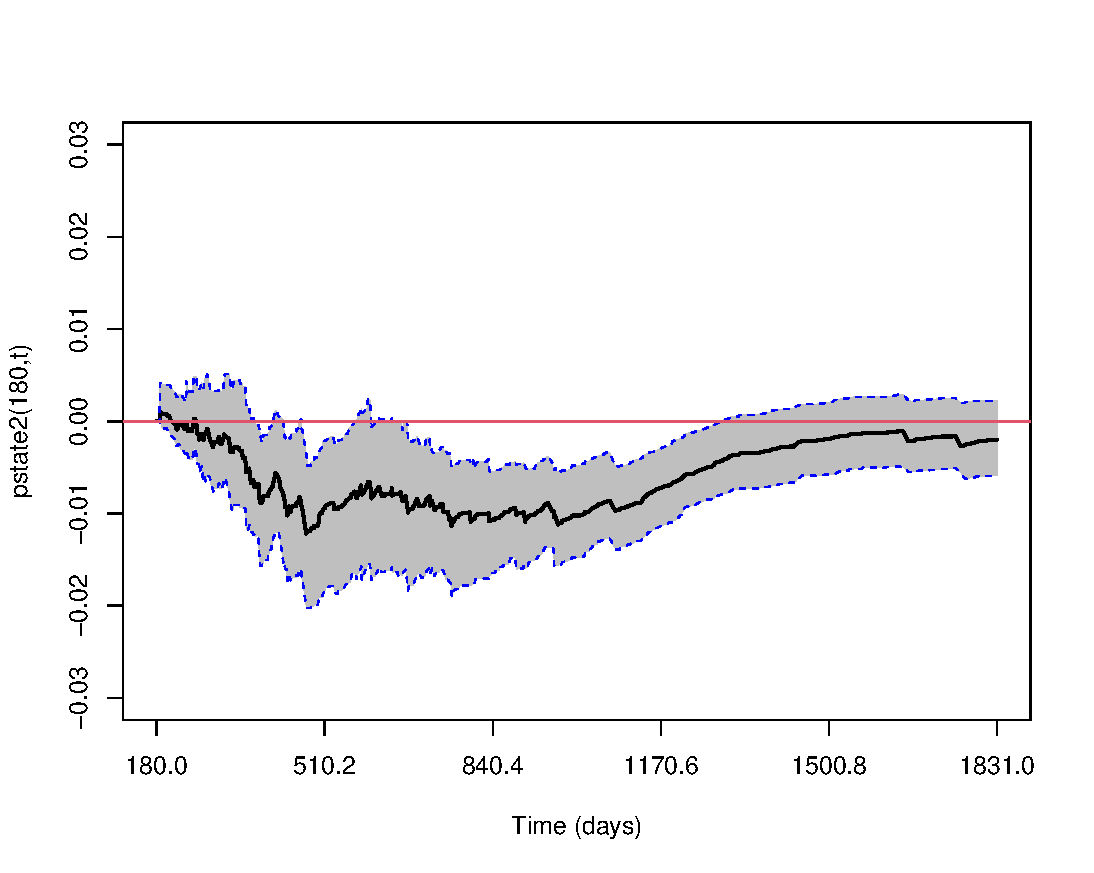
\includegraphics[width=6.5cm, height=6.5cm]{Fig6/1_t180_new2.pdf}
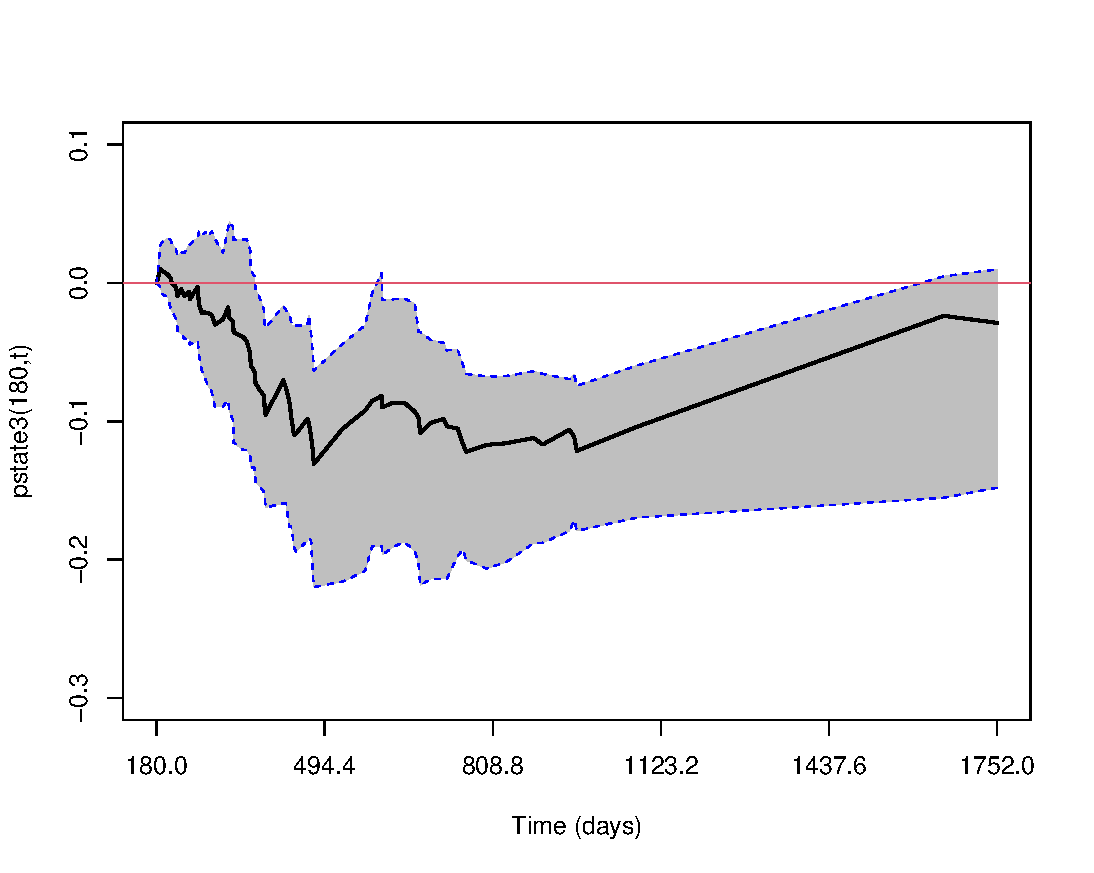
\includegraphics[width=6.5cm, height=6.5cm]{Fig6/2_t180_new2.pdf}\\

\caption{A local graphical test for the Markov condition for colon cancer data, for $s = 180$, based on the discrepancy between the Aalen-Johansen estimator (Markovian) and the Markov-free estimator (\texttt{LMAJ}) for each time from \textit{s}. Bootstrap resamples were used to determine the 95\% confidence interval.}
\label{fig6}
\end{center}
\end{figure}

The plots in Figure \ref{fig6} can be thought of as graphical local tests for the Markov assumption. As expected, in both cases they reveal differences between the two methods for $s=180$ since they show a clear deviation with respect to the horizontal line $y=0$. From these, one gets some (graphical) evidence of the lack of Markovianity of the underlying process beyond half a year after surgery. Therefore, for this specific time, the application of the Aalen-Johansen method may not be recommended here, due to possible biases. %They also reveal a possible failure of the Markov assumption.

In Section 2, a global test was also introduced that combines the probability values of the local test over different times (given by the percentiles of the sojourn time in State 1). In the \CRANpkg{markovMSM} package, this can be obtained using the function \code{AUC.test}. The arguments for this function are described in Table~\ref{Tab3}. Some examples of how to perform the proposed AUC global test are shown in the following input commands, in which we consider the default percentiles in the argument \texttt{quantiles}. Depending on the number of replicas, the implementation of the \code{AUC.test} function can be computationally time-consuming.

%{\color{red} o nome da função pode levar a confusão pois temos também o teste global pelo modelo de cox e pelo LR. Sugestão: AUC.test esta função pode proporcionar os resultados do teste local e global pelo método AUC.}

%{\color{red} tal como está para os testes locais poderia colocar no output dos testes globais as respetivas transições em cima.}

%\begin{CodeInput}
\begin{example}
> set.seed(1234)
> res4 <- AUC.test(data = db_long, from = 1, to = 3, type = 'global', replicas = 100, 
                   tmat = tmat)    
           
> round(res4$globalTest,3)
   1->1  1->2  1->3
1 0.067 0.012 0.012

> set.seed(1234)
> res5 <- update(res4, from = 2) 
> round(res5$globalTest,3)
    2->3
1  0.006 
\end{example}
%\end{CodeInput}


Results reported by the first command lines provide the probability values for the global test based on the AUC for the three transitions leaving State 1 (i.e., $1\rightarrow 1$, $1\rightarrow 2$ and $1\rightarrow 3$). As expected, a higher probability value was obtained for transition 1$\rightarrow$1 than the two remaining transitions, revealing evidence against the Markov condition. Results reported in the second set of input commands agree with previous findings, reporting a probability value of 0.006 for 2$\rightarrow$3. Among the objects saved by this function, \code{AUC.test} displays the probability values for each percentile time (default to 5, 10, 20, 30, and 40) through the following codes:


%\begin{CodeInput}
\begin{example}
> round(res4$localTest,3)
      s    1->1   1->2   1->3
1  102.4  0.978  0.081  0.081
2  173.0  0.118  0.025  0.025
3  290.6  0.015  0.000  0.000
4  469.2  0.679  0.056  0.056
5  726.8  0.635  0.176  0.176

> round(res5$localTest,3)
    s     2->2   2->3
1 102.4   0.015  0.015
2 173.0   0.011  0.011
3 290.6   0.000  0.000
4 469.2   0.050  0.050
5 726.8   0.156  0.156
\end{example}
%\end{CodeInput}


These outputs show, for instance, that the probability value of the AUC local test reveal the fail of the Markovian assumption for the third percentile time ($p$-value < 0.001). Plots with the graphical local tests for the respective quantiles can be easily obtained using the following input commands:

%\begin{CodeInput}
\begin{example}
> plot(res4, quantileOrder = 3, to = 2, axis.scale = c(-0.04, 0.02))
  #Figure 4 (Left column)

> plot(res5, quantileOrder = 3, to = 3, axis.scale = c(-0.20, 0.10))
  #Figure 4 (Right column)
\end{example}
%\end{CodeInput}

\begin{figure} [t] %[h!]
\begin{center}
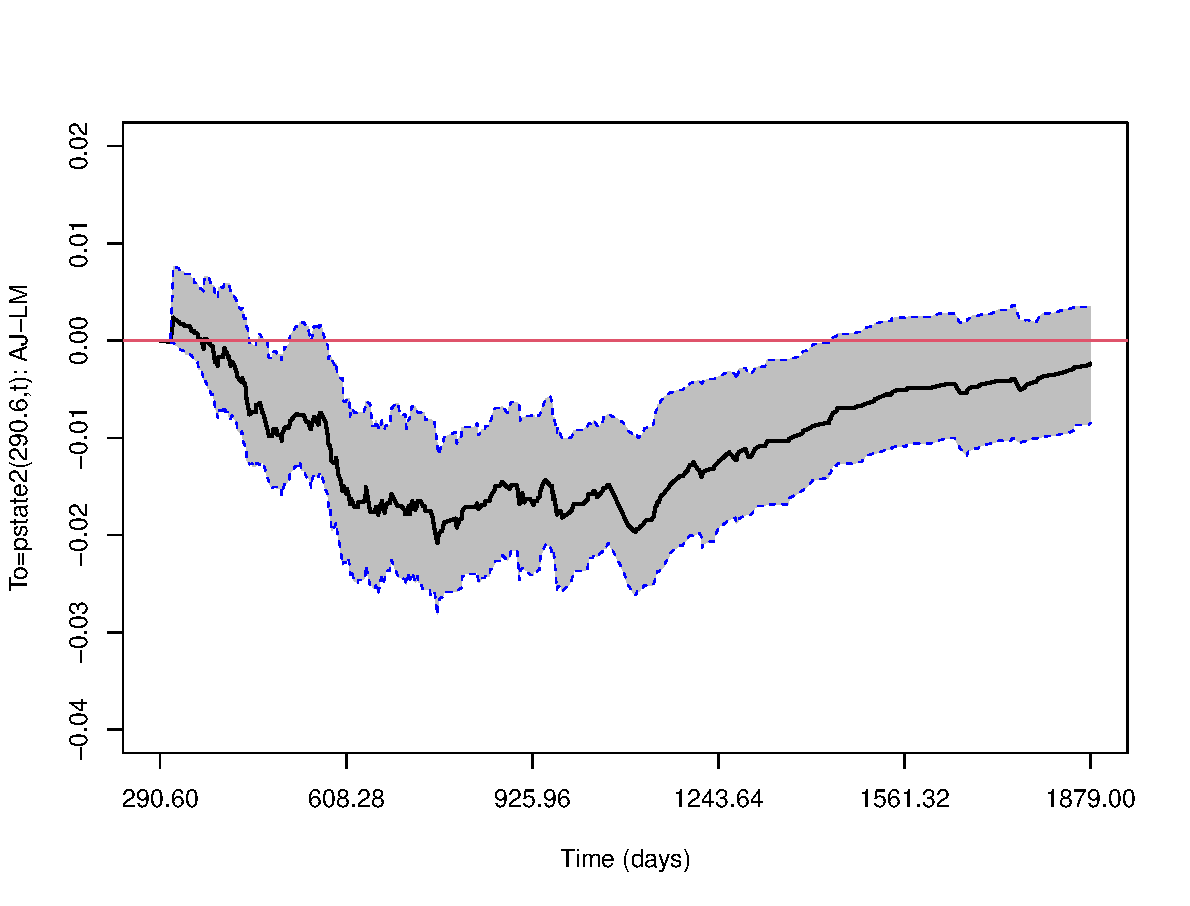
\includegraphics[width=6.5cm, height=6.5cm]{survIDM-images/perc3_p12_new3_final.pdf}
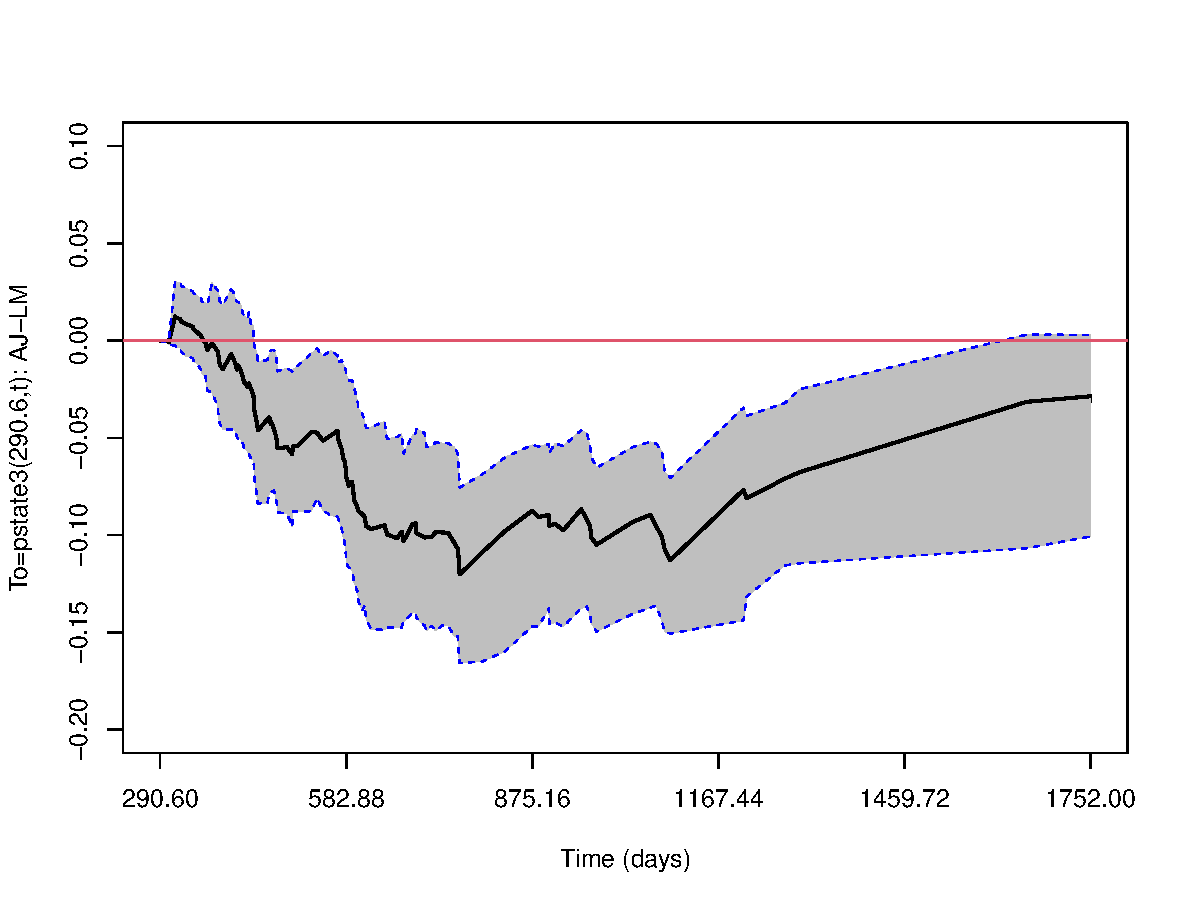
\includegraphics[width=6.5cm, height=6.5cm]{survIDM-images/perc3_p23_new3_final.pdf}\\
\caption{Local graphical test for the Markov condition for colon cancer data, for \textit{s} equal to 290.6, the third percentile of the sojourn time in the initial state. Transition 1$\rightarrow$2 is shown on the left hand side, and transition 2$\rightarrow$3 is shown on the right hand side.}
\label{fig8}
\end{center}
\end{figure}

The plots shown in Figure \ref{fig8} display the differences between the \code{AJ} and \code{LMAJ} estimates for the third quantile (\code{quantileOrder}) of the sojourn time in the initial state being in accordance with the \textit{p}-values obtained in the local tests.

%{\color{red} tal como apontado atras na funcao para o teste pelo modelo de cox, nao me parece boa ideia o argumento transition tal como esta pois o utilizador vai ter dificuldade em saber o que é a transição 3. Sugestão: transition="23" ou from=2, to=3.}

Often, multi-state models include covariates, and it may be the omission of covariate effects that induces apparent non-Markovianity. The methods proposed in this paper can also deal with this problem since discrete covariates can be included in the estimation of the transition probabilities $p_{hj}(s, t)$ by splitting the sample for each level of the covariate and repeating the described procedures for each subsample. As an example, the following input codes show how to obtain the AUC global for individuals with the treatment `Obs’ of covariate `rx'. To this end, we start to filter the wide data set \texttt{colonMSM} and run the \code{prepMSM} function to obtain the subgroups of the new data in the format long. At least, we just need to use the \code{AUC.test} function for the specific transitions as follows:

\begin{example}
> db_wide_obs <- db_wide[db_wide$rx == 'Obs',]
> db_long_obs <- prepMSM(data = db_wide_obs, trans, timesNames, status)
> set.seed(12345)
> res4.obs <- AUC.test(data = db_long_obs, times = 365, from = 1, to = 3, 
                       type='local', replicas = 100, tmat = tmat)
> res4.obs$localTest

    s      1->1         1->2         1->3
1 365   0.6295861   0.0003563306  0.0004307342

> set.seed(12345)
> res5.obs <- AUC.test(data = db_long_obs, times = 365, from = 2, to = 3, 
                       type = 'local', replicas=100, tmat = tmat)
> res5.obs$localTest

    s         2->2         2->3
1  365    5.935795e-05  0.0001894722
\end{example}
%> AUC.test(db_long, db_wide, from=1, to=3, type='local', replicas=100, tmat = tmat)


The \CRANpkg{markovMSM} package can also be used to compute the results of the global and local tests proposed by \cite{Titman2020} which are based on log-rank statistics. A summary of the arguments of the \code{LR.test} function is shown in Table~\ref{Tab4}. The following input commands illustrate the usage of \code{LR.test} function to implement these tests:

%\begin{CodeInput}
\begin{example}
> set.seed(1234)
> res6 <- LR.test(data = db_long, times = 180, from = 2, to = 3, replicas = 1000)
> res6$globalTestLR
  [1] 0.047
\end{example}
%\end{CodeInput}


%{\color{red} rever o paragrafo em baixo. Será que não seria melhor omitir res7 pois está de certa forma em contradição com res6. Repare que para s=180 obtemos 0.026 e para s=173 0.113. Ficaria apenas com res6 e juntava o comando para o teste global a partir de res6} {\color{blue} Retirei res7, assim como o texto que estava associado a res7}

As we can see, the probability value of the global tests based on the log-rank statistics confirms the possible failure of Markovianity for lower values of $s$ (P=0.047 < 0.05).

\begin{table}[t!]%[h]
\begin{small}
\begin{tabular}{p{3.5cm}p{9.6cm}}
%\toprule
\hline
Argument & Description \\
\hline
%\midrule
\code{data} & Multi-state data in \code{msdata} format, which is created from the \texttt{mstate} package. It should also contain (dummy coding of) the relevant covariates; no factors allowed.\\
\code{times} & Grid of time points at which to compute the statistic.\\
\code{from} & The starting state of the transition to check the Markov condition.\\
\code{to} & The last state of the considered transition to check the Markov condition.\\
\code{replicas} &  The number of wild bootstrap replications. This method, proposed by \cite{Wu1986} is commonly applied to solve problems related to heterocedasticity. \cite{Beyersmann2012} found better small sample results using centered Poisson random variables rather than standard normal weights. For further information on the usage of the wild bootstrap, see \cite{Titman2020}.\\
\code{formula} & Right-hand side of the formula. If \code{NULL} will fit with no covariates (formula="1" will also work), offset terms can also be specified.\\
\code{fn} &  A list of summary functions to be applied to the individual zbar traces (or a list of lists).\\
\code{fn2} & A list of summary functions to be applied to the overall chi-squared trace.\\
\code{dist} &  Distribution of wild bootstrap random weights, either \code{poisson} for centred Poisson (default), or \code{normal} for standard normal.\\
\code{min\_time} &  The minimum time for calculating optimal weights.\\
\code{other\_weights} & Other (than optimal) weights can be specified here.\\
%\bottomrule
\hline
\end{tabular}
\caption {Summary of the arguments of the function \code{LR.test}.}
\label{Tab4}
\end{small}
\end{table}
%\newpage 


\subsection{Tests for Markov assumption for more complex multi-state models} \label{sec:mkv tests1}

In this section, we use two data sets to illustrate the extension of the previous functions to more complex multi-state models. As a first example, we consider the data of 2279 patients transplanted by the European Society for Blood and Marrow Transplantation (EBMT) and, as a second example, data from liver cirrhosis patients subjected to prednisone treatment. Further details on the description of the data can be found in \cite{Putter2007} and \cite{Andersen1993}, respectively. 

The steps taken in the analysis are quite similar to those introduced for the illness-death model. To extend the proposed local and global tests to more complex models, we make use of the \code{LMAJ} estimator that produces consistent estimates of the transition probabilities in the case of non-Markovianity of the process.

We start by considering the data set comprising 2279 patients who suffered from blood cancers and who were treated at the EBMT between 1985 and 1998 after a transplant. The movement of the patients among the six states can be modeled through the multi-state model with the following six states: `Alive and in remission, no recovery or adverse event' (state 1); `Alive in remission, recovered from the treatment' (state 2); `Alive in remission, occurrence of the adverse event' (state 3); `Alive, both recovered and adverse event' (state 4); `Alive, in relapse' (treatment failure) (state 5) and `Dead (treatment failure)' (state 6). In total, there are 12 transitions: three intermediate events given by recovery (Rec), adverse event (AE) and a combination of the two (AE and Rec), and two absorbing states: relapse and death (Figure~\ref{fig9b}).

\begin{figure}[t] %[h!]
\centering
%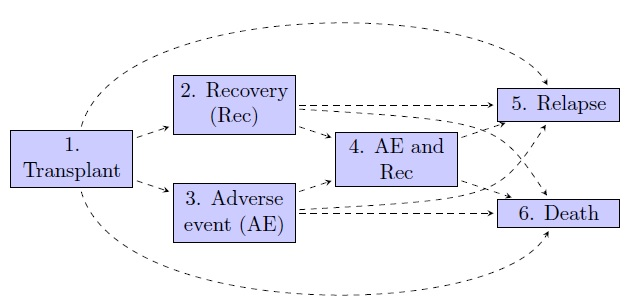
\includegraphics[width=9.5cm]{ebmt4-model.jpg}
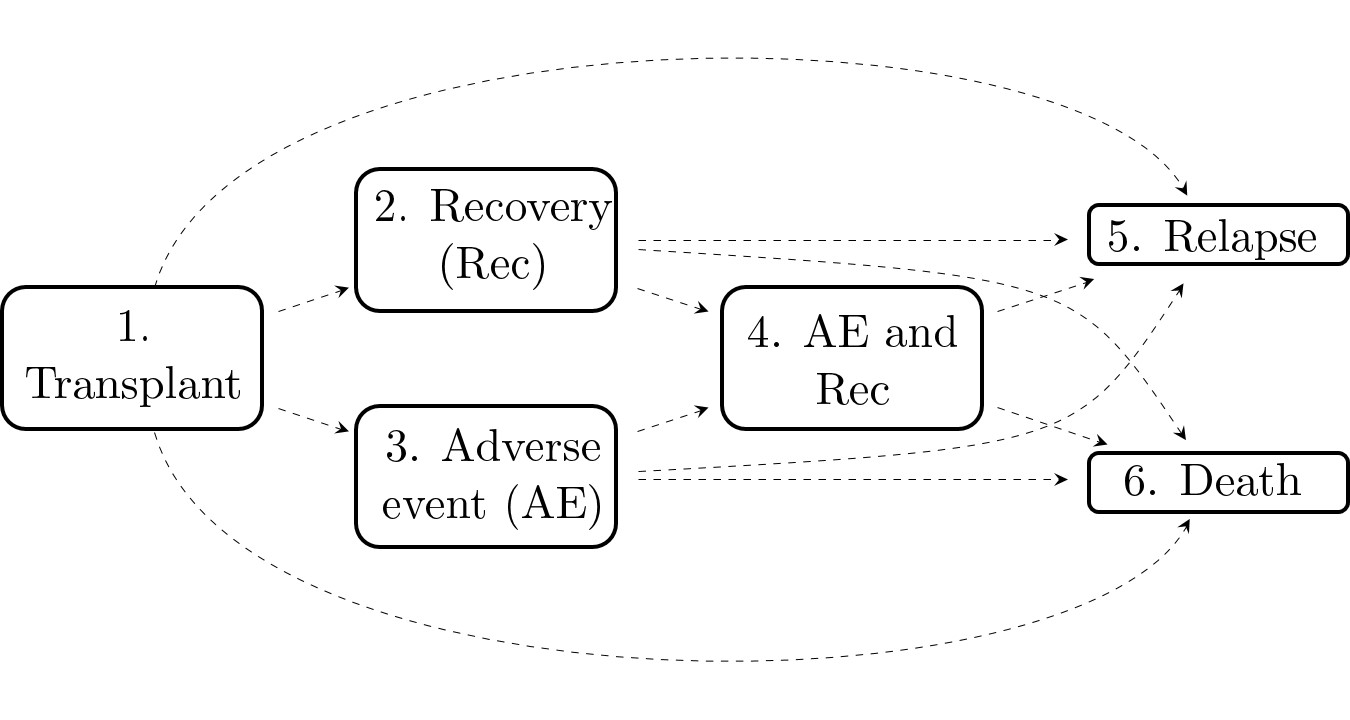
\includegraphics[width=10cm]{bmt_model2.jpg}
\caption {A six-state model given by the Blood and Marrow Transplantation (EBMT) data set for leukemia patients after bone marrow transplantation.} 
\label{fig9b}
\end{figure}

Since the original data \code{ebmt4} is in the wide format, before implementing a global test we need to convert it into the long format using functions \code{transMatMSM}, \code{prepMSM} before using function \code{AUC.test} with the argument \code{type='global'}:

%\begin{CodeInput}
\begin{example}
> data("ebmt4")
> db_wide <- ebmt4
> positions <- list(c(2, 3, 5, 6), c(4, 5, 6), c(4, 5, 6),
                 c(5, 6), c(), c())
> state.names <-  c("Tx", "Rec", "AE", "Rec+AE", "Rel",  "Death")
> tmat <- transMatMSM(positions, state.names)
> timesNames <- c(NA, "rec", "ae","recae", "rel", "srv")
> status <- c(NA, "rec.s", "ae.s", "recae.s","rel.s", "srv.s")
> trans <- tmat
> db_long <- prepMSM(data = db_wide, trans, timesNames, status)
> db_long[1:10,]

Data:
   id from to trans Tstart Tstop time status
1   1    1  2     1      0    22   22      1
2   1    1  3     2      0    22   22      0
3   1    1  5     3      0    22   22      0
4   1    1  6     4      0    22   22      0
5   1    2  4     5     22   995  973      0
6   1    2  5     6     22   995  973      0
7   1    2  6     7     22   995  973      0
8   2    1  2     1      0    12   12      0
9   2    1  3     2      0    12   12      1
10  2    1  5     3      0    12   12      0

> set.seed(1234)
> res7 <- AUC.test(data = db_long, from = 1, to = 5, type = 'global',
        quantiles = c(0.05, 0.10, 0.20, 0.30, 0.40),
        tmat = tmat, replicas = 100,
        positions = positions, namesStates = state.names,
        timesNames = timesNames, status = status)
        
        
                  
> round(res7$globalTest, 4)
    1->1    1->2    1->3   1->4    1->5
1  0.1417 0.0094 0.0231 0.099 0.0068

> round(res7$localTests,4)
     s   1->1   1->2   1->3   1->4   1->5
1  9.9 0.2822 0.6030 0.0176 0.0848 0.0137
2 12.0 0.2833 0.5230 0.0285 0.4643 0.0000
3 15.0 0.0001 0.2106 0.0398 0.0191 0.1193
4 18.0 0.4584 0.0041 0.1763 0.1789 0.0240
5 21.0 0.0060 0.0147 0.4673 0.2363 0.4796
\end{example}
%\end{CodeInput}


%{\color{red} Não percebo a necessidade do argumento to=5 em res8. Na minha opinião, neste caso apenas deveriamos obter o valor de prova para p15(s,t). Caso não se coloque o argumento "to" deveria dar para todas as transições a partir de 1. Como creio que está! Atenção que na ultima parte do output não está claro o que é pstate4 e pstate5. Na realidade é a transição de 1 para 5 e 1 para 6. Por isso ficaria mais claro se em cima tivessemos "11", "12", "13", "15" e "16". Isto em todas as funções. Consegue obter isso no from e no to.} {\color{blue} Professor Luís, aqui segui a ideia da biblioteca mstate no qual from=1 to=5 permite obter todas as probabilidades de transição possíveis entre 1 e 5. Neste caso calcula todos os testes para essas transições}

%{\color{red} O memmo comentário que coloquei em cima. As correções melhoraram substancialmente a biblioteca. Um detalhe, caso ainda seja possível alterar. Colocar no res7\$globalTest as transições em cima também.}

The interpretation of the output for the global test and for local tests of the five percentile times is similar to that shown for the illness-death model. Thus, object \code{res7} is used to get a list with components giving the probability values for the Markov test for all transitions leaving State 1 (i.e., for 1$\rightarrow$ j with $j\in \{1,2,3,4,5\}$). For instance, the probability value of 0.0094 corresponds to the result of the AUC global test for transition 1$\rightarrow$2, while 0.0147 is the probability value for the local test, for $s=21$ for the same transition. 

The proposed methods can also be used in reversible multi-state models such as those applied to the data set of liver cirrhosis patients who were included in a randomized clinical trial at several hospitals in Copenhagen between 1962 and 1974. The study aimed to evaluate whether a treatment based on prednisone prolongs survival for patients with cirrhosis \cite{Andersen1993}. State 1 corresponds to `normal prothrombin level', State 2 to `low (or abnormal) prothrombin level', and State 3 to `dead'. The movement of the patients among these three states can be modeled using the reversible illness-death model shown in Figure~\ref{fig9}. The input commands for the local and global tests of the AUC and Log-rank tests are presented as a vignette in the \texttt{markovMSM} package.


\begin{figure}[t] %[h!]
\centering
%\includegraphics[width=12.5cm]{prothr-model.jpg}
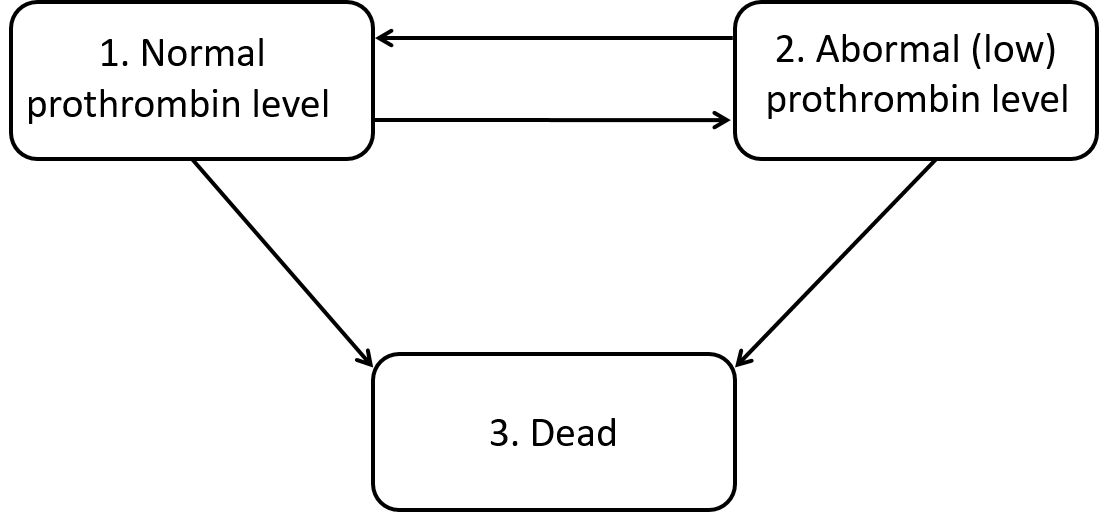
\includegraphics[width=6.5cm]{IDM_liver.pdf}
\caption {A reversible illness-death model from the data set of patients with liver cirrhosis subjected to prednisone treatment. Reversible transitions are possible in transient states defined by prothrombin levels.} \label{fig9}
\end{figure}


\section{4. Conclusions} \label{sec:conc}
This paper discusses the implementation in R of new methods for checking the Markov assumption in multi-state models proposed by \cite{soutinho_machado2020}. Instead of testing, as usual, the Markovianity of the multi-state process by including covariates depending on the history, \cite{soutinho_machado2020} propose global and local tests based on the comparison between estimated transition probabilities. This can be done by measuring the discrepancy between the Aalen-Johansen estimator, which gives consistent estimators in Markov processes, and recent approaches that do not rely on this assumption, given by the Landmark and the Landmark Aalen-Johansen estimators. 

The use of local tests is recommended whenever the goal is to estimate the transition probabilities and, in particular, decide which estimator is the most appropriate to use: the Aalen-Johansen estimator or a robust estimator. A global test, such as the test proposed here, might be preferable for regression purposes. To this end, a common simplifying strategy is to decouple the whole process into various survival models. Then, for all permitted transitions, the transition intensities may be modeled using separate Cox models, assuming the process to be Markovian (also known as the clock forward modeling approach). When the test rejects the Markov assumption, one alternative approach is to use a semi-Markov Cox model in which the future of the process does not depend on the current time but rather on the duration of the current state.

A brief summary of the theory underlying these methods has been provided, along with an extensive review of the current literature. A detailed usage of the three main functions that compose the \CRANpkg{markovMSM} package, \code{AUC.test}, \code{LR.test} and \code{PHM.test} are illustrated using three real data sets: \code{colonIDM}, \code{ebmt4} and \code{prothr}. Whereas the first data enables the application of the Markov tests to an illness-death model, the last two cases show how to extend the proposed methods to more complex multi-state models (with more than three states or with reversible transitions). The comparison of the proposed tests to the new methods given by the log-rank test described by \cite{Titman2020} is also shown. We also present approaches to validate the suspicion of the failure of the Markovianity of the process using graphical tests. The \CRANpkg{markovMSM} package is available at the first author's GitHub repository as well as the CRAN repository at https://cran.r-project.org/web/packages/markovMSM. Further details on the usage of its functions can be obtained from the corresponding help pages.


%[From Titman] Note that the local log-rank test statistic in (3.1) will be undefined or unstable in time periods in which very few patients are either in, or not in, the qualifying state j.As such, [t0, tmax] should be chosen to avoid periods, typically at the beginning or end of follow-up, where this may occur. A

\section*{Acknowledgments}
This research was financed by Portuguese Funds through FCT - "Funda\c{c}\~{a}o para a Ci\^{e}ncia e a Tecnologia", within Projects projects UIDB/00013/2020, UIDP/00013/2020 and the research grant PD/BD/142887/2018.\\

%This research was financed by Portuguese Funds through FCT - "Funda\c{c}\~{a}o para a Ci\^{e}ncia e a Tecnologia", within the research grant PD/BD/142887/2018. Lu\'{i}s Meira-Machado acknowledges financial support from the Spanish Ministry of Economy and Competitiveness MINECO through project MTM2017-82379-R funded by (AEI/FEDER, UE) and acronym "AFTERAM".\\

\bibliography{paper}

\address{Gustavo Soutinho\\
EPIUnit\\
  Institute of Public Health of the University of Porto (ISPUP)\\
  Rua das Taipas 135, 4050-600 Porto\\
  Portugal\\
  ORCID: 0000-0002-0559-1327\\
  \email{gdsoutinho@gmail.com}}

\address{Lu\'{i}s Meira-Machado\\
  Department of Mathematics \& Centre of Mathematics\\ University of Minho\\
  Campus de Azur\'{e}m - 4800-058 Guimar\~{a}es\\
  Portugal\\
  ORCID: 0000-0002-8577-7665\\
  \email{lmachado@math.uminho.pt}}

